\documentclass{article}

\usepackage[english]{babel}
\usepackage{hyperref, float, amsmath, amssymb}
\usepackage{tikz, xcolor, ifthen}
\usepackage{caption, subcaption}
\usepackage{pgfplots, accents}
\usepackage[inline,shortlabels]{enumitem}

%\usepackage[list=off]{caption}

\usetikzlibrary{ fit, calc, arrows, shapes }

\newcommand{\red}[1]{{\color{red} #1}}
\newcommand{\green}[1]{{\color{green} #1}}
\newcommand{\yellow}[1]{{\color{yellow} #1}}



\begin{document}

% \begin{abstract}  % TODO
% \emph{University classes scheduling} is an old, well-known problem, that
% was attacked by the researches only recently, as the advances in electronics,
% made in the last 10--15 years, permitted construction of computational
% systems, far more advanced than \red{\dots}
% \end{abstract}

% Solutions to the problem are the \emph{university schedules}, that are
% composed of \emph{individual schedules} for each \emph{group} (\emph{student}),
% \emph{professor} and \emph{classroom}.

% Individual schedules are represented by \emph{timetables}, that hold one's
% \emph{classes} for a week. % TODO: rewrite this!
% A \emph{class} denotes some activity for a group of students under professor's
% supervision, that takes place in the classroom assigned. Actual activity and
% therefore the requirements, imposed on both professor and classroom, are defined by the
% \emph{discipline} in question.

\begin{abstract}

University classes scheduling problem consists in assigning
the \emph{classes}, defined by the academic program, for
each group of students, possibly taking in account participants' interests.

The problem is solved by agents negotiation over possible classes
configurations. The \emph{negotiating agents} are grouped by \emph{roles}:
\emph{professors} (\emph{full} and \emph{part time}), \emph{students} (\emph{groups}) and
\emph{classrooms}. Each agent has the knowledge, required by it's role.

The \emph{configuration} quality is assessed by it's \emph{coherence}.
A solution must exceed some quality threshold.

\end{abstract}

\bigskip
\tableofcontents
\newpage

\documentclass[ThesisDoc]{subfiles}
\begin{document}

\section{Introduction}

\todo


\end{document}

%\documentclass{article}


%\usepackage{xcolor, amsmath}
%\newcommand{\red}[1]{{\color{red} #1}}


\def\coh{\mathrm{coh}}

\def\restrC{\accentset{C}{\xi}^p_i}
\def\restrT{\accentset{T}{\xi}}
\def\restrS{\accentset{S}{\xi}^p_i}
\def\restrW{\accentset{W}{\xi}^p_i}

%\begin{document}

\section{Problem Formalization}

Let \begin{itemize}
\item $D=\{d_i\}$ be the set of \emph{disciplines}.
  A discipline may be seen as class descriptor, it contains
  academic program name and information about special requirements,
  such as laboratories.
\item $G=\{g_i\}$ be the set of \emph{groups}.
  A group unites some students. In this thesis it is assumed that
  \textbf{each student belongs strictly to one group}.
  A group has a set of disciplines, that it is obliged to take by an
  academical program.
\item $P=\{p_i\}$ be the set of \emph{professors}.
  Each professor can teach a set of disciplines, that is determined
  by the institution. There are two kinds of professors:
  \emph{full-time} and \emph{part-time}. The difference is that the
  latter have more flexible obligations, while the former have preference
  in classes assignment.
\item $R=\{r_i\}$ be the set of \emph{classrooms}.
  A classroom has two properties: capacity and special equipment installed.
\item $D=\{\bar d_i\}$ be the set of working \emph{days}.
\item $T=\{t_i\}$ be \emph{discrete time} (limited by working hours).
\item $ c \sim \left< d, g, p, r, \bar d, t_b, t_e \right> $ be a \emph{class}
  of discipline $d$ for group $g$, taught by professor $p$, that takes place
  at classroom $r$ every day $d$ in time interval $t_b$--$t_e$.
\item $\{\restrC\}$ be the restrictions over classes of participant $p$.
      $\restrC : c \mapsto \mathrm{Bool}$
\item $\restrT$ be the \emph{time-consistency} restriction, that ensures
  classes non-intersection for each participant.
      $\restrT : c \mapsto c \mapsto \mathrm{Bool}$
\item $\{\restrS\}$ be the rest of strong restrictions, or \emph{obligations},
      of participant $p$.
      $\restrS : \{c\} \mapsto \mathrm{Bool}$
\item $\{\restrW\}$ be the weak restrictions, or \emph{preferences}, of participant $p$.
      In order to avoid overrestrictions, the preferences should weaken with time.
      $\restrW : \tau \mapsto \{c\} \mapsto (0,1]$
% \item $\xi^p$ be the combined restrictions of agent $p$.
\item $\tau$ be \emph{negotiation time}. $\tau \in \mathbb{N}$
\end{itemize}
\medskip

A \emph{candidate} to solution $\tilde{c}$ is a configuration (set) of classes
$\{c\}$, that form participant's individual schedule. An \emph{acceptable candidate}
respects all the restrictions $\{\xi^p_i\}$ (of the participant $p$),
thus can be selected as the solution (individual).
% $\tilde{c}^+ | \forall c \in \tilde{c}^+ $
\bigskip

\noindent
Restrictions compliance is assessed with \emph{coherence},
$\coh[a]: \tilde c \mapsto \Re$
that is properly discussed in \ref{sectionCoherence}.
It defines an order over the candidates and permits
agents to extract the \emph{acceptable} ones using a threshold.


The coherence function is designed in such a way, that given a candidate,
each agent, mentioned by candidate's underlying classes, yields the same
coherence assessment for the candidate.


\begin{align}
  \label{eq:coh-fun-independ}
  \begin{aligned}
    &\forall \tilde{c} = \{c_k\} \\
    &\forall c_i \sim \left< \dots, g_i, p_i, r_i, \dots \right> \\
    &\forall c_j \sim \left< \dots, g_j, p_j, r_j, \dots \right>
  \end{aligned}
& \implies
  \begin{aligned}
   \coh[g_i](\tilde c) &= \coh[g_j](\tilde c) = \\
   = \coh[p_i](\tilde c) &= \coh[p_j](\tilde c) = \\
   = \coh[r_i](\tilde c) &= \coh[r_j](\tilde c)
  \end{aligned}
\end{align}







%\end{document}

%\documentclass{article}


%\usepackage{hyperref, float, amsmath}
%\usepackage{tikz, ifthen, xcolor}
%\usepackage[english]{babel}

%\usetikzlibrary{fit, calc, arrows, shapes}

%\newcommand{\red}[1]{{\color{red} #1}}


%\begin{document}

\def\coh{\mathrm{coh}}
\def\cohi{\mathrm{\widetilde{coh}}}


\section{Coherence}
\label{sec:Coherence}

\subsection{Coherence theory}

\begin{displayquote}
Coherence theory is a psychologically motivated motivational cognitive theory with
foundations in philosophy that approaches problems in terms of the satisfaction
of multiple constraints within networks of highly interconnected elements
\cite[p.~19]{UAB-Thesis}.
\end{displayquote}

\red{
In the \cite{UAB-Thesis}, it actually references
[Thagard, 2002, Thagard, 2006], but I don't know if it's a direct quotation from
there (it sounds like); so, I don't know what reference should I put,
on Thagard or the \cite{UAB-Thesis}?}

It can be understood in terms of maximal satisfaction of multiple
constraints \cite{ThagVerb98}
\red{it's also an almost direct quotation, should I format it as one?}.
According to \cite{ThagVerb98}, the method can be used to solve problems in
diverse areas, such as logic, mathematics, law, ethics, rationality, etc.


In Thagard's theory, the coherence problem is about partitioning a graph of
\emph{information pieces}, interconnected by positive or negative weighted
constraints, that enhance or diminish partition's coherence.
The coherence-maximizing partition is the one that has maximum number of constraints
satisfied.


The best partition $\mathcal{A}$ \red{(called \emph{candidate} in this thesis)}
of graph  $\mathcal{V}$  is obtained, considering both
$\mathcal{A}$ (accepted pieces) and
$\mathcal{V} \backslash \mathcal{A}$ (rejected pieces) \cite{ThagVerb98}.

\medskip

\noindent

An example of partitioning by Thagard's method is given in figure \ref{fig:UAB-partition}.
The information graph $\mathcal{V}$ consists of
classes $C_1,\dots,C_4$, also there are three possibilities for
class $C_1$ placement and two for class $C_4$. A relation is
\begin{itemize}[leftmargin=3cm]
  \item[\red{\emph{inconsistent}}], if two classes intersect in time;
  \item[\yellow{\emph{same class}}], if two classes differ only by time;
  \item[\green{\emph{consistent}}], otherwise.
\end{itemize}

\noindent
The coherence of the partition $\mathcal{A},\mathcal{V}\backslash\mathcal{A}$
          is calculated as
\medskip

$   \dfrac{ \text{\green{\emph{consistent}} relations in } \mathcal{A}
          + \text{\red{\emph{inconsistent}} relations between }
                  \mathcal{A} \text{ and } \mathcal{V}\backslash\mathcal{A}}
          {\text{total relations in } \mathcal{V}}$.
\medskip

\noindent
It's value is $\frac{|1| \cdot 3 + |-1| \cdot 5}{17} \approx 0.47$.


\begin{figure}[h]
  \centering
  \includegraphics[width=0.5\textwidth]{img/UAB-splitting.png} % scale=0.5
  % \captionsetup{singlelinecheck=off}
  \caption{Example: information graph partitioning, proposed by Thagard
           \cite{ThagVerb98, UAB-Thesis}. }
  \label{fig:UAB-partition}
\end{figure}


\subsection{Coherence and Contexts}
\label{section:coherence}

In PHD thesis \cite{UAB-Thesis}, the author establishes concrete
\emph{coherence functions}, based on the properties, proposed by Thagard for
such functions. The author chooses \emph{g-BDI} agent architecture ---
a \emph{multi-context} system, where the contexts are: \emph{beliefs},
\emph{desires} and \emph{intentions}. Each context has its \emph{internal rules}
for computing context's logics and there are \emph{bridge rules} that allow to
import contexts' results into other contexts. It should be noted, that \emph{g-BDI}
architecture uses \emph{fuzzy logics}.

The \emph{information graph} is obtained by joining contexts' graphs with the
help of \emph{bridge rules}  \cite[62]{UAB-Thesis}.

\bigskip


\noindent
In this thesis, a different aproach is taken. The initial information graph,
composed of \emph{classes propositions}, is passed to a \emph{splitting} context,
that generates all posiible \emph{acceptable} (by the splitting context) sub-graphs,
called \emph{candidates} (as it will be shown in \emph{Beliefs} context).

Each candidate is propagated through the contexts in the established
order. At each context it gets assessed
(using \emph{context-specific} knowledge and relations)
and the result is compared against \emph{context-specific threshold}.
If passing threshold test,
the candidate is sent to the next context, otherwise it is marked as failed
(providing a reason) and is propagated no further. In both cases the coherence
value is guarded alongside the candidate.

Thus a context in this thsis serves as \emph{candidates} filter. This approach
allows us to avoid:
\begin{enumerate}
  \item Usage of \emph{bridge rules}. It permits more flexebility for
    the \emph{internal rules}. Changes in contexts' logics do not affect the way
    the results are combined, even if the changes are incompatible.
  \item Huge graph partitioning. Such graph would have to unite all the
    candidates and every context's internal knowledge. Then the entire graph
    needs to be stored, until the best partition is found.

    In \red{my} approach, both \emph{candidates generation} and
    \emph{filtering} can be done sequentially and lazily,
    thereby cutting memory usage.

\end{enumerate}

\medskip

\noindent
A \emph{context} represents an aspect for optimization/restriction, considered
by an agent. It defines context-specific information and relations over the
information graph, with the corresponding combination functions. There are
two types of relations: \emph{binary} and over the \emph{whole graph}. The former ones
are applied to every pair of nodes and the results are combined by
\emph{binary fold functions} (one combines the results of the same relation
and the other combines the latter results). The whole-graph relations' values are
combined by the corresponding \emph{whole-graph fold function}. In the end the
combined values of both relations types are merged into the result by
\emph{combined merge function}. All the combination functions are defined at
contexts.

\begin{figure}[h]
  \centering
  \fbox{ \input{../src/Document/tikz/ContextAssess} }
  \caption{Binary relations within an information graph. One can
           distinguish the relations between the assessed information pieces
           and the relations between assessed and the known ones.
          }
\end{figure}

\subsection{Internal Contexts}

An internal context requires no knowledge from other agents.
The combined coherence of all the internal contexts is called
\emph{inner coherence} and is denoted as $\cohi$.

% % % % % % % % % % % % % % % % % % % % % % % % % % % % % % % % % % % % % % % %
\subsubsection{Capabilities}

Represent \emph{strong} restrictions, imposed by the institution.
All the relations should yield
\begin{itemize}
  \item [1], if the restriction is satistied;
  \item [0], otherwise.
\end{itemize}

The threshold for this context is $1$.
All types of restrictions are combined by \emph{multiplication}, thus
any broken condition would cause zero result.


Institution restrictions:
\begin{itemize}
\item \textbf{Group:} the candidate has the correct amount of classes for each
  discipline inscribed.
\item \textbf{Professor:} can teach every discipline assigned.
\item \textbf{Classroom:} has enough capacity and meets all special requirements.
\end{itemize}

An agent should be keeping the capabilities of known agents, to avoid creation
of unacceptable classes.

\begin{figure}[h]
  \centering
  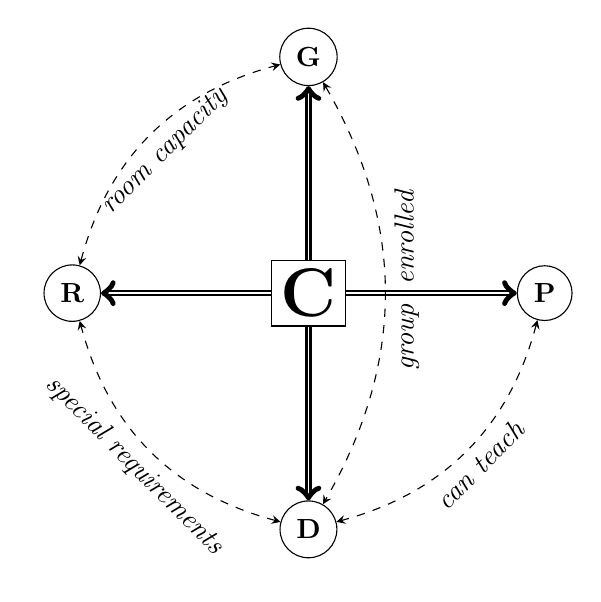
\begin{tikzpicture}

\edef\r{3cm}

\node[draw]         (C) at (0,  0) {\textbf{\Huge C}};
\node[draw, circle] (G) at (0, \r) {\textbf{G}};
\node[draw, circle] (P) at (\r, 0) {\textbf{P}};
\node[draw, circle] (D) at (0,-\r) {\textbf{D}};
\node[draw, circle] (R) at (-\r,0) {\textbf{R}};

\foreach \i in {(G),(P),(D),(R)}
 \draw[->, thick, double] (C) -- \i;

\def\data{ P/D/can teach
         , D/R/special requirements
         , R/G/room capacity
         , G/D/\quad group~~enrolled
         }

\foreach \i/\j/\k in \data
 \draw[<->, >=stealth, dashed] (\i) to[bend left
                                      ,edge node={node [sloped, below] {\emph{\k}}}]
                               (\j);


\end{tikzpicture}

  \caption{Capabilities required to form a \emph{class}.}
  \label{fig:capabilities}
\end{figure}


% % % % % % % % % % % % % % % % % % % % % % % % % % % % % % % % % % % % % % % %
\subsubsection{Beliefs (Time Consistency)}

Asserts that all the classes (concerning the assessing agent), are consistent in
time (do not intersect). This context is a splitting one, it uses the time
consistence relation to generate all possible time-consistent candidates from
given classes. It's internal knowledge should hold \emph{classes pool}, that
would be used for candidates generation via \emph{graph splitting}.
\\

The \emph{time consistence} relation yields following values:
\begin{itemize}[leftmargin=2cm]
  \item[-1], if two classes intersect in time (are inconsistent);
  \item[0], if two classes differ only by time
            (while have same discipline, group, professor and classroom);
  \item[1], otherwise (are consistent).
\end{itemize}


The splitting process uses context's relation \emph{aggregation} strategy.

\begin{align*}
  \mbox{Let } & C=\lbrace c \rbrace \text{ be the \emph{classes pool}}.\\
            ~ & A_i=\lbrace a_i \rbrace \text{ be a set of \emph{acceptable candidates},
                                         composed of } i \text{ classes.}\\
            ~ & A=\bigcup\limits_{i} A_i \text{ be a set of \emph{acceptable candidates}}.
\end{align*}

\begin{enumerate}
  \item Each single-class candidate is acceptable:
    $A_1 = \lbrace [ c ] ~||~ \forall ~ c \in C \rbrace$.
  \item Form $A_2$ by extending each candidate $[c'] = a_1 \in A_1$ with $c \in C$,
    if and only if $c'$ and $c$ are \emph{consistent in time}.
    If $A_1 \not= \emptyset$, then try to form $A_2$.
  \item[\vdots]
  \item[i.] Form $A_i$ by extending each candidate $[c'_1, \dots, c'_{i-1}] = a_{i-1}
    \in A_{i-1}$ with $c \in C$, if and only if $\forall c' \in a_{i-1}, ~c'$
    and $c$ are \emph{consistent in time}.
    If $A_i \not= \emptyset$, then try to form $A_{i+1}$.
   \item[\vdots]
   \item[n.] $A_n = \emptyset \implies$ all the \emph{acceptable candidates}
     were generated. Done.
\end{enumerate}


\begin{figure}[h]
  \label{fig:splittingCtx}
  \def\sfwidth{0.24\textwidth}
  \begin{subfigure}[b]{\sfwidth}
    \includegraphics[width=\textwidth]{img/split-1-class.png}
    \caption{All single-class candidates are acceptable.}
  \end{subfigure}
  \begin{subfigure}[b]{\sfwidth}
    \includegraphics[width=\textwidth]{img/split-2-class_1.png}
    \caption[caption]{$\begin{aligned}
              A_3^2    &= A_1^1 + A_4^1\\
              A_2^2    &= A_2^1 + A_6^1\\
              A_{10}^2 &= A_3^1 + A_7^1
            \end{aligned}$}
  \end{subfigure}
  \begin{subfigure}[b]{\sfwidth}
    \includegraphics[width=\textwidth]{img/split-2-class_2.png}
    \caption[caption]{$\begin{aligned}
              A_1^2 &= A_2^1 + A_4^1\\
              A_4^2 &= A_1^1 + A_7^1\\
              A_8^2 &= A_5^1 + A_6^1
             \end{aligned}$}
  \end{subfigure}
  \begin{subfigure}[b]{\sfwidth}
    \includegraphics[width=\textwidth]{img/split-2-class_3.png}
    \caption[caption]{$\begin{aligned}
              A_5^2    &= A_1^1 + A_5^1\\
              A_{11}^2 &= A_3^1 + A_5^1\\
              A_6^2    &= A_4^1 + A_6^1
             \end{aligned}$}
  \end{subfigure}
\\
  \begin{subfigure}[b]{\sfwidth}
    \includegraphics[width=\textwidth]{img/split-2-class_4.png}
    \caption[caption]{$\begin{aligned}
              A_7^2 &= A_4^1 + A_7^1\\
              A_9^2 &= A_3^1 + A_6^1
             \end{aligned}$}
  \end{subfigure}
  \begin{subfigure}[b]{\sfwidth}
    \includegraphics[width=\textwidth]{img/split-3-class_1.png}
    \caption[caption]{$\begin{aligned}
              A_1^3 &= A_2^2 + A_4^1\\
                    &= A_1^2 + A_6^1\\
                    &= A_6^2 + A_2^1
              \end{aligned}$}
  \end{subfigure}
  \begin{subfigure}[b]{\sfwidth}
    \includegraphics[width=\textwidth]{img/split-3-class_2.png}
    \caption[caption]{$\begin{aligned}
              A_2^3 &= A_3^2 + A_7^1\\
                    &= A_4^2 + A_4^1\\
                    &= A_7^2 + A_1^1
              \end{aligned}$}
  \end{subfigure}
  \begin{subfigure}[b]{\sfwidth}
    \includegraphics[width=\textwidth]{img/split-3-class_3.png}
    \caption[caption]{$\begin{aligned}
              A_3^3 &= A_8^2    + A_3^1\\
                    &= A_{11}^2 + A_6^1\\
                    &= A_9^2    + A_5^1
              \end{aligned}$}
  \end{subfigure}

  \caption{Information graph \emph{splitting} example. The graph is the same
           as in figure \ref{fig:UAB-partition}.
           There are in total \textbf{7}  1-class candidates,
                                    \textbf{11} 2-class candidates and
                                    \textbf{3}  3-class candidates.}
\end{figure}



% % % % % % % % % % % % % % % % % % % % % % % % % % % % % % % % % % % % % % % %
\subsubsection{Obligations}

The obligations determine custom \emph{strong restrictions} over the classes.
As in the case of \emph{capabilities}, the obligation relations must yield a
boolean result. The threshold in this context is $1$ and the restrictions are
combined by \emph{multiplication}.


Possible \emph{obligation relations} examples: maximum classes per day,
lunch recess time, lower/upper class time limit, two classes must/cannot follow etc.

\red{At the moment there are no obligations used (but they are supported).}

% % % % % % % % % % % % % % % % % % % % % % % % % % % % % % % % % % % % % % % %
\subsubsection{Preference}

The preferences define \emph{weak restrictions}. The relations values might be any
value within $[0,1]$ interval. To avoid overrestrictions, this context's \emph{threshold}
should decrease with time. The binary and whole-graph relations are combined
using \emph{mean} operation; the two results are combined by sum. The
\emph{initial threshold value}, as well as preference threshold \emph{decrease rate}
must be explicitly provided.

\red{Possible preferences}

\subsection{External}

The external context asks counterparts an \emph{opinion} about a candidate.
An opinion is the \emph{inner coherence} of the agent being asked. This context
plays crucial role in coherence property \ref{eq:coh-fun-independ}. It combines
the internal coherences of the agent itself and other agents, mentioned in the
assessed candidate.

To speedup opinions assessment, the agents should share the newly created classes.
Any class $c_i \sim \left< \dots, g_i, p_i, r_i, \dots \right>$, created by
any agent of triple $\left< g_i, p_i, r_i \right>$, should be sent by that
agent to the rest of the triple. A received class must be added to agent's
classes pool.

\begin{figure}[h]
  \label{fig:CandidatesShareOpinions}
  \includegraphics[width=\textwidth]{img/CandidatesShareOpinions.png}
  \caption{Agents exchange thier \emph{internal coherences} of the candidates
            $\cohi^a_i = \cohi[a](c_i)$ in form \emph{opinions}.
          }
\end{figure}

The internal coherences are combined using \emph{common goal} function $\Gamma$.
The common goal must combine three coherence values (from a group, professor and
classroom), making no difference between value origins.
$$
  \Gamma(\coh_x^G, \coh_x^P, \coh_x^R) = \Gamma(\coh_x^G, \coh_x^R, \coh_x^P)
    = \dots = \Gamma(\coh_x^R, \coh_x^P, \coh_x^G)
$$

The simplest \emph{common goal} functions are \emph{product} $\prod$
and \emph{mean} $\frac{\sum_n}{n}$.


\red{The $\Gamma$ function ensures \ref{eq:coh-fun-independ} coherence property,
that permits to avoid \dots}


%\end{document}

%\begin{document}


% \def\lifetime    {\mathit{lifetime}}
% \def\class       {\mathit{class}}
% \def\execute     {\mathit{execute}}
% \def\decide      {\mathit{decide}}
% \def\knownClasses{\overset{\mathrm{known}}{\mathit{classes}}}


\section{Agents}

The \emph{negotiating agents} are isolated proactive computational entities,
capable of sending and receiving messages.
The \emph{isolation} denotes that agents' internal states are protected
from outside access. Messaging is the only way an agent can be interacted with.
The \emph{pro-activity} implies a capacity of acting asynchronously,
with no ``external'' cause.

\medskip

An agent is defined by it's behaviour --- the combination of its
\emph{proactive} and \emph{reactive} (message handling) functions.

Therefore two agents with same behaviour functions should be considered two instances
of the same agent. In must be noted, that all the diference in the behaviour of
two instances is produced by the differences in the states
(both agent's internal state and the environment's one).

\medskip

In order to generalize agents behaviour, agent \emph{roles} are introduced.
A role describes whom or what an agents represents in the negotiation and
defines \emph{behaviour archetype} --- the rules to build
agent's \emph{behaviour functions}, given some \emph{role-specific} knowledge.

\subsection{Agents Implementation}

Agents are implemented using \emph{Software Transactional Memory} (STM)
\cite{STMCode07} --- a promising concurrency paradigm.
They are executed in two computational threads:
one for message handling and another for proactive action.

\medskip

\noindent
Agent's behavior is flexible and may be changed during agent's lifetime.
As it was mentioned before, it is determined by \emph{message handling} and
\emph{action} functions.
Any complex behaviour would require the agent to have some \emph{mutable}
internal \emph{states}, where it could store the related information,
thus remembering it throughout behaviour executions.
The only restriction is that states interface must be fixed for type safety
(only the interface, not the underlying data).


Each agent also has two system states: the \emph{run state} and special \emph{shared
  state}, called \emph{status}. The run state controls agent's execution
(and termination), while the status is monitored by the respective controller.
Agents have three \emph{run states}: ``Paused'', ``Running'' and ``Terminate''.
The first two states should control pro-action;
setting the last one should cause all agent's processes to stop.
The \emph{status}es are further described in section \ref{agentControllers}.

\medskip

To ensure agents isolation, the direct interactions are restricted;
an agent only exposes its communication interface through \emph{agent reference}.

Using this interface, one can simply \emph{send} a message to an agent,
or one can \emph{ask} for some \emph{expected response}, corresponding to the message sent.
Agents have separate handler functions for theese two cases.

\medskip

All behavior functions
accept two arguments:
\begin{enumerate}
\item the agent's \emph{inner interface}, that provides
  control over agent's own behavior and lifetime;
\item agent's \emph{internal state}.
\end{enumerate}

\subsubsection{Negotiation}


A negotiation has a \emph{classes pool}, distributed between the agents.
A class $\left< d, g, p, r, \bar d, t, t \right>$ is known to agents,
representing $g$, $p$ and $r$.

Negotiations are organized by special kind of agents --- \emph{controllers}.

\red{TODO}


\subsubsection{Coherence-based}

\red{ They are not the same as ``Coherence-driven Agents'' from \cite{UAB-Thesis}!
      It should be properly described.
 }

A \emph{coherence-based agent} bases its decisions on existing \emph{candidates}
and their \emph{coherence}. It must contain it's contexts within the state,
define contexts order and set the splitting one. It also must provide a
\emph{decider}.
\medskip

\noindent
Such agent acts repeatedly:
\begin{enumerate}
\item Gets its \emph{classes pool}, that may be stored within some context or
  somewhere else in the state.
\item Generates the initial candidates, using the \emph{splitting context} and
  classes pool.
\item Propagates the candidates through the contexts, as described in section
  \ref{section:coherence}.
\item Passes the \emph{assessed candidates} to the \emph{decider}.
\end{enumerate}

The decider must choose between two actions:
\begin{itemize}
\item Add new class(es) to the \emph{pool}. Such decision is taken if
  none of assessed candidates is \emph{acceptable}.
\item Select best solution and wait. This should be done if a satisfying
  solution was found. The agent's \emph{run state} is set to ``Paused'' and
  the \emph{status} is updated to ``Waiting''.
\end{itemize}

\subsubsection{Classes generation}
\label{section:class-gen}
When no \emph{acceptable candidates} can be obtained by combining the classes
from the \emph{pool}, new class need to be added (to the \emph{classes pool}).

In order to avoid ``garbage'' classes generation, the newly created classes must:
\begin{enumerate}[(1)]
  \item Be \emph{capacity} consistent. The group, professor and classroom,
    assigned to the class, must be \emph{capable} of handling the assigned discipline
    (it must comply with their respective \emph{capabilities}).
  \item Not be a repetition of any of \emph{discarted classes}
    (see section \ref{section:clean-pool}).
\end{enumerate}

In order to keep track of discarted classes without keeping them around,
class \emph{hashes} may be used. The only restriction on hash function is
injectiveness:
\begin{align*}
  \forall c_1, c_2 \in \text{ \emph{classes}} & \\
  \mathrm{hash}(c_1) &= \mathrm{hash}(c_2) \implies c_1 = c_2
\end{align*}

\subsubsection{Pool cleanup}
\label{section:clean-pool}

Even with no discipline-inconsistent classes being genrated
(sec. \ref{section:class-gen} (1)), the amount of
``bad'' classes (that worsen solutions) would be growing.
Those classes need to be discarted and their \emph{hashes} guarded
to be used in \ref{section:class-gen} (2). Discarted classes hashs must be
shared between \emph{group}, \emph{professor} and \emph{classroom} agents,
corresponding to the class.

A class should be considered \emph{solution worsening} and be discarted, if
\begin{enumerate}
  \item no \emph{acceptable candidate} (after propagating through all the contexts)
    contains the class;
  \item \red{?}
\end{enumerate}


\red{TO DO}





\subsection{Controllers}

The controllers create new negotiating agents, and monitor their \emph{status}es
over their lifetimes. Controllers also provide communication references for the
agents they control. In order to facilitate references sharing, the controllers
are restricted to a single \emph{role} for it's agents.

Controllers have hierarchical structure, starting with the \emph{root
  controller}. The orders received by \emph{root} are propagated to
the underlying controllers.

\medskip

As mentioned before, negotiating agents have a special state,
called \emph{status}, that is monitored by the controllers. Apart
from receiving agents' errors, the \emph{status}es are used to
extract the \emph{distributed solution} from the agents.
This is done using ``Waiting'' and ``Locked'' statuses.

The agents set ``Waiting'' status when a suitable solution is found,
and the corresponding controller waits for all of its subjugated
agents to set it. When it is done, the controller sends ``Lock''
command to the agents and notifies the \emph{parent controller}.
When the \emph{root controller} receives ``Lock'' notifications from
all the controllers, it sends ``Collect'' order. On that order, the controllers
extract the solution parts (guarded in the statuses) and propagate them up to
the root.


\newpage
\bibliographystyle{plain}
\bibliography{references}

\end{document}
